%LTeX: language=pt-br
% !TeX root = Apostila_IM381.tex

\newpage
\subsection{Elementos retangular e quadrado}
\label{app:el_retangular}

    Na Seção \ref{sec:isoparametrico}, descrevemos a formulação completa de um elemento isoparamétrico quadrangular qualquer. Neste apêndice, verificaremos o caso particular de um elemento retangular. Considere o elemento de comprimento $b$ e altura $h$ da Figura \ref{fig:el_retangular}. Note que, embora este elemento esteja fixado na coordenada $(0,0)$, as conclusões que chegaremos não dependem da posição dele no espaço, isto é, o primeiro nó poderia ocupar qualquer posição, desde que os outros transladassem proporcionalmente.

    \begin{figure}[h!]
        \centering
        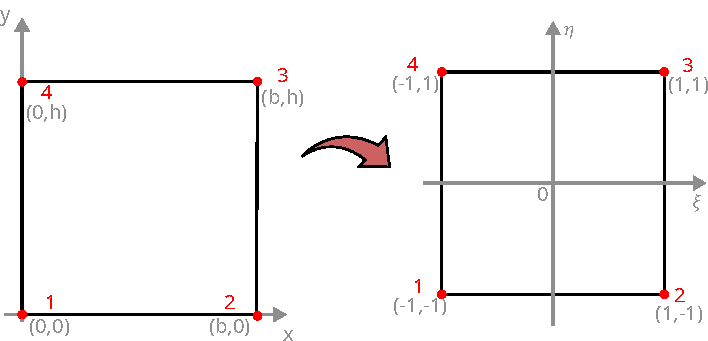
\includegraphics[scale=1]{Figures/Apendice/Retangulo.pdf}
        \caption{Elemento retangular com dimensões $b$ e $h$.}
        \label{fig:el_retangular}
    \end{figure}

    Tanto as funções de forma quanto o Jacobiano deste elemento permanecerão iguais ao caso geral mostrado anteriormente. Portanto, substituindo as coordenadas dos nós nas expressões das derivadas das coordenadas globais em relação às locais:

    \begin{equation*}
        \frac{\partial x}{\partial \xi} = \frac{b}{2}
    \end{equation*}

    \begin{equation*}
        \frac{\partial x}{\partial \eta} = 0
    \end{equation*}

    \begin{equation*}
        \frac{\partial y}{\partial \xi} = 0
    \end{equation*}

    \begin{equation*}
        \frac{\partial y}{\partial \eta} = \frac{h}{2}
    \end{equation*}

    Portanto:

    \begin{equation}
        \mathbf{J} = 
        \begin{bmatrix}
                \frac{b}{2} &  0\\
                0 &  \frac{h}{2}
        \end{bmatrix}
    \end{equation}

    \begin{equation}
        \det \mathbf{J} = 
        \frac{bh}{4}
    \end{equation}

    \begin{equation}
        \mathbf{J}^{-1} = 
        \frac{4}{bh}\begin{bmatrix}
                \frac{h}{2} &  0\\
                0 &  \frac{b}{2}
        \end{bmatrix}=
        \begin{bmatrix}
                \frac{2}{b} &  0\\
                0 &  \frac{2}{h}
        \end{bmatrix}
    \end{equation}

    As derivadas das funções de forma em relação às coordenadas globais:

    \begin{equation}
        \begin{Bmatrix}
            \frac{\partial N_i}{\partial x} \\
            \frac{\partial N_i}{\partial y}
        \end{Bmatrix} = 
        \mathbf{J}^{-1}
        \begin{Bmatrix}
            \frac{\partial N_i}{\partial \xi} \\
            \frac{\partial N_i}{\partial \eta}
        \end{Bmatrix}
    \end{equation}


    \begin{equation}
        \begin{Bmatrix}
            \frac{\partial N_1}{\partial x} \\
            \frac{\partial N_1}{\partial y}
        \end{Bmatrix} = 
        \mathbf{J}^{-1}
        \begin{Bmatrix}
            \frac{\partial N_1}{\partial \xi} \\
            \frac{\partial N_1}{\partial \eta}
        \end{Bmatrix}=
        \begin{bmatrix}
                \frac{2}{b} &  0\\
                0 &  \frac{2}{h}
        \end{bmatrix}
        \begin{Bmatrix}
            -\frac{1}{4}\left(1-\eta\right) \\
            -\frac{1}{4}\left(1-\xi\right)
        \end{Bmatrix}=
        \begin{Bmatrix}
            -\frac{1}{2b}\left(1-\eta\right) \\
            -\frac{1}{2h}\left(1-\xi\right)
        \end{Bmatrix}
    \end{equation}

    \begin{equation}
        \begin{Bmatrix}
            \frac{\partial N_2}{\partial x} \\
            \frac{\partial N_2}{\partial y}
        \end{Bmatrix} = 
        \mathbf{J}^{-1}
        \begin{Bmatrix}
            \frac{\partial N_2}{\partial \xi} \\
            \frac{\partial N_2}{\partial \eta}
        \end{Bmatrix}=
        \begin{bmatrix}
                \frac{2}{b} &  0\\
                0 &  \frac{2}{h}
        \end{bmatrix}
        \begin{Bmatrix}
            \frac{1}{4}\left(1-\eta\right) \\
            -\frac{1}{4}\left(1+\xi\right)
        \end{Bmatrix}=
        \begin{Bmatrix}
            \frac{1}{2b}\left(1-\eta\right) \\
            -\frac{1}{2h}\left(1+\xi\right)
        \end{Bmatrix}
    \end{equation}

    \begin{equation}
        \begin{Bmatrix}
            \frac{\partial N_3}{\partial x} \\
            \frac{\partial N_3}{\partial y}
        \end{Bmatrix} = 
        \mathbf{J}^{-1}
        \begin{Bmatrix}
            \frac{\partial N_3}{\partial \xi} \\
            \frac{\partial N_3}{\partial \eta}
        \end{Bmatrix}=
        \begin{bmatrix}
                \frac{2}{b} &  0\\
                0 &  \frac{2}{h}
        \end{bmatrix}
        \begin{Bmatrix}
            \frac{1}{4}\left(1+\eta\right) \\
            \frac{1}{4}\left(1+\xi\right)
        \end{Bmatrix}=
        \begin{Bmatrix}
            \frac{1}{2b}\left(1+\eta\right) \\
            \frac{1}{2h}\left(1+\xi\right)
        \end{Bmatrix}
    \end{equation}

    \begin{equation}
        \begin{Bmatrix}
            \frac{\partial N_4}{\partial x} \\
            \frac{\partial N_4}{\partial y}
        \end{Bmatrix} = 
        \mathbf{J}^{-1}
        \begin{Bmatrix}
            \frac{\partial N_4}{\partial \xi} \\
            \frac{\partial N_4}{\partial \eta}
        \end{Bmatrix}=
        \begin{bmatrix}
                \frac{2}{b} &  0\\
                0 &  \frac{2}{h}
        \end{bmatrix}
        \begin{Bmatrix}
            -\frac{1}{4}\left(1+\eta\right) \\
            \frac{1}{4}\left(1-\xi\right)
        \end{Bmatrix}=
        \begin{Bmatrix}
            -\frac{1}{2b}\left(1+\eta\right) \\
            \frac{1}{2h}\left(1-\xi\right)
        \end{Bmatrix}
    \end{equation}

    Essas derivadas são lineares, seja em $\xi$, seja $\eta$. A matriz $\bm{B}$, portanto, também terá a mesma forma. Finalmente, a matriz de rigidez será dada por:

    \begin{equation}
        \mathbf{K}_e = \int_\Omega  \mathbf{B}^T \mathbf{D} \mathbf{B} dA = \int_{-1}^{1} \int_{-1}^{1}  \mathbf{B}^T \mathbf{D} \mathbf{B} \det \mathbf{J} d\xi d\eta
    \end{equation}

    A função dentro da integral ($\mathbf{B}^T \mathbf{D} \mathbf{B} \det \mathbf{J}$), terá grau 2 em $\xi$ e grau 2 em $\eta$. Isto ocorre pois $\bm{B}$ tem grau 1, $\bm{D}$ e $ \det \mathbf{J}$ têm grau 0. Desta forma, é necessário um grid de pelo menos $2 \times 2$ pontos de Gauss para integração exata:

    \begin{equation}
        N_\xi \geq \frac{P_\xi+1}{2} = \frac{2+1}{2} = 1,5
    \end{equation}

    \begin{equation}
        N_\eta \geq \frac{P_\eta+1}{2} = \frac{2+1}{2} = 1,5
    \end{equation}

    É possível abrir esta expressão analiticamente, entretanto, esta fica bastante complicada e com vários termos extensos, sendo preferível ou a abertura destas uma única vez através de bibliotecas simbólicas de programação, ou a integração numérica.

    Para ilustrar a abertura explícita destas expressões, simplificaremos mais ainda a formulação do elemento, considerando um elemento quadrado, com $b=h=l$. Portanto, a matriz $\bm{B}$ deste elemento fica:

    \begin{equation}
        \mathbf{B} = 
        \frac{1}{2l}\begin{bmatrix}
            -\left(1-\eta\right) & 0 & \left(1-\eta\right) & 0 & \left(1+\eta\right) & 0 & -\left(1+\eta\right) & 0 \\
            0 & -\left(1-\xi\right) & 0 & -\left(1+\xi\right) & 0 & \left(1+\xi\right) & 0 & \left(1-\xi\right)\\
            -\left(1-\xi\right) & -\left(1-\eta\right) & -\left(1+\xi\right) & \left(1-\eta\right) & \left(1+\xi\right) & \left(1+\eta\right) & \left(1-\xi\right) & -\left(1+\eta\right)\\
        \end{bmatrix}
    \end{equation}

    \begin{equation}
        \mathbf{B} = 
        \frac{1}{2l}\begin{bmatrix}
            -f_1(\eta) & 0 & f_1(\eta) & 0 & f_2(\eta) & 0 & -f_2(\eta) & 0 \\
            0 & -f_1(\xi) & 0 & -f_2(\xi) & 0 & f_2(\xi) & 0 & f_1(\xi)\\
            -f_1(\xi) & -f_1(\eta) & -f_2(\xi) & f_1(\eta) & f_2(\xi) & f_2(\eta) & f_1(\xi) & -f_2(\eta)\\
        \end{bmatrix}
    \end{equation}

    \noindent nos quais $f_1$ e $f_2$ foram definidos para simplificar as operações.

    A matriz de rigidez fica, considerando estado plano de tensão:

    \begin{equation}
        \mathbf{K}_e = \int_\Omega  \mathbf{B}^T \mathbf{D} \mathbf{B} dA = \int_{-1}^{1} \int_{-1}^{1}  \mathbf{B}^T \mathbf{D} \mathbf{B} \det \mathbf{J} d\xi d\eta
    \end{equation}

    \begin{multline}
        \mathbf{K}_e \int_{-1}^{1} \int_{-1}^{1}  
         \frac{1}{2l}\begin{bmatrix}
            -f_1(\eta) & 0 & -f_1(\xi)\\
            0          & -f_1(\xi) & -f_1(\eta)\\
            f_1(\eta) & 0 & -f_2(\xi)\\
            0          & -f_2(\xi) & f_1(\eta)\\
            f_2(\eta) & 0 & f_2(\xi)\\
            0          & f_2(\xi) & f_2(\eta)\\
            -f_2(\eta) & 0 & f_1(\xi)\\
            0          & f_1(\xi) & -f_2(\eta)
        \end{bmatrix} 
        \frac{E}{1-\nu^2}
        \begin{bmatrix}
            1 & \nu & 0\\
            \nu & 1 & 0\\
            0 & 0 & \frac{1-\nu}{2}
        \end{bmatrix}\\
        \frac{1}{2l}\begin{bmatrix}
            -f_1(\eta) & 0 & f_1(\eta) & 0 & f_2(\eta) & 0 & -f_2(\eta) & 0 \\
            0 & -f_1(\xi) & 0 & -f_2(\xi) & 0 & f_2(\xi) & 0 & f_1(\xi)\\
            -f_1(\xi) & -f_1(\eta) & -f_2(\xi) & f_1(\eta) & f_2(\xi) & f_2(\eta) & f_1(\xi) & -f_2(\eta)\\
        \end{bmatrix} 
        \frac{l^2}{4} d\xi d\eta
    \end{multline}

    \begin{equation}
        \mathbf{K}_e = \int_\Omega  \mathbf{B}^T \mathbf{D} \mathbf{B} dA = \int_{-1}^{1} \int_{-1}^{1}  \mathbf{B}^T \mathbf{D} \mathbf{B} \det \mathbf{J} d\xi d\eta
    \end{equation}

    Utilizando a biblioteca simbólica Sympy, podemos chegar em:

    \begin{equation}
        \mathbf{K}_e = 
        \frac{E}{16\left(1-\nu^2\right)}\begin{bmatrix}
            2a & b  & c  & d  & -a & -b & e  & -d\\
            b  & 2a & -d & e  & -b & -a & d  & c \\
            c  & -d & 2a & -b & e  & d  & -a & b \\
            d  & e  & -b & 2a & -d & c  & b  & -a\\
            -a & -b & e  & -d & 2a & b  & c  & d \\
            -b & -a & d  & c  & b  & 2a & -d & e \\
            e  & d  & -a & b  & c  & -d & 2a & -b\\
            -d & c  & b  & -a & d  & e  & -b & 2a\\
        \end{bmatrix}
    \end{equation} 
 
    \noindent nos quais, para simplificar, foram definidas as variáveis:

    \begin{equation*}
        a = 4 - \frac{4\nu}{3}
    \end{equation*}

    \begin{equation*}
        b = 2\nu + 2
    \end{equation*}

    \begin{equation*}
        c = -\frac{4\nu}{3} - 4
    \end{equation*}

    \begin{equation*}
        d = 6\nu - 2
    \end{equation*}
    
    \begin{equation*}
        e = \frac{8\nu}{3}
    \end{equation*}

    Note que, ao contrário do que nossa intuição, a matriz de rigidez de um elemento quadrado não depende de suas dimensões.